\section{Backend} \label{back}
In this section we illustrate the design and implementation of the backend of compiler of $\lambda_Q$.
The backend consists of four parts: lexer, parser, qubit allocation and optimization.
\subsection{Lexer \& Parser}
We use Lex/Yacc to implement the lexer and parser of a modified version of OpenQasm2.0 in backend.

Subcircuit definition is not available in our OpenQasm2.0. Besides $\{U3,CX\}$ that are available in the original OpenQasm2.0, we add $\{H,X,Y,Z\}$ to the built-in gate set.

This part consists of 600 lines of C code formatted in Lex/Yacc file's syntax.
Readers can refer to \textit{lex.l} and \textit{parser.y} to get more detailed information.

\subsection{Qubit allocation}
In recent years, some companies like IBM have made quantum computers available to wide community.
Users can build their experiments based on a circuit representation on the cloud platform. However, today's quantum computer prototypes have tight resources constraints.
For instance, you can only apply two qubits operations to a subset of qubit pairs which is specificed by a partial network.

In \textit{qubit\_allocation.cpp}, we implement a heuristic algorithm  to allocate physical qubits to logic qubits.

\subsubsection{Problem Definition}
The most basic form of Qubit Allocation Problem is: given a quantum circuit and an architecture, we want to know if it is possible to map logic qubits in the former to physical qubits in the latter.
Notice that even this basic form problem is already NP-hard.

In some cases, the constraints of the architecture is impossible to satisfy, and we need some circuit transformation to relax these constraints.

There are three kinds of transformation we can apply:
\begin{itemize}
    \item[Reversal] Apply $CX$ to $(p,q)$ when $(q,p)$ is available in the architecture.
    \item[Bridge] Apply $CX$ to $(p,q)$ when $(p,s)$ and $(s, q)$ is available.
    \item[Swap] Swap the state of $p$ and $q$ when $(p,q)$ or $(q,p)$ is available.
\end{itemize}

All these transformation need extra gates to implement, so we need to find a qubit mapping and circuit transformations to satisfy the constraints with minimum number extra gates involved.

\subsubsection{Algorithm}

Our algorithm has two stages:

\textbf{First stage}: Find an intial mapping

We first sort the logic qubits in descending order of their occurrence counts.

Then, for each logic qubit $q$ in order, we allocate $q$ to a physical qubit with the nearest out-degree(both the quantum circuit and the architecture can be regarded as a directed graph whose vertex is qubits)

After $q$ is allocated to $p$, for each edge $(q,q')$, we try to allocate $q'$ to some $p'$ with edge $(p,p')$ and has the nearest out-degree.

Repeat the above process for $q'$ if it is successfully allocated.

After this BFS-like allocation we allocate the rest unallocated logic qubit to a free physical qubit.

\textbf{Second stage}: Adjust the mapping and apply circuit transformation

The mapping $l$ in the output of the first stage may not satisfy all constraints, so we need to adjust it and apply circuit transformations to the quantum circuit.

For any two qubit operation on $(p,q)$, if $(l(p),l(q))$ can't be implemented in current mapping, then:
\begin{itemize}
    \item[1.] if $(p,q)$ appears more than once in the circuit, we use a Swap transformation to move $q$ closer to $p$ (Here we can use BFS to find the shortest path to $p$) and then re-evaluate these four cases.
    \item[2.] else if $(l(q), l(p))$ can be implemented, then we use a Reversal transformation to $l(q)$ and $l(p)$.
    \item[3.] else if $\exists s$ s.t. $(l(p),s)$ and $(s, l(q))$ are both available, we can use a Bridge transformation to $l(p), s, l(q)$.
    \item[4.] else use Swap transformation like case 1.
\end{itemize}
\subsection{Optimization}

Optimization for arbitary unitary gates is sophisticated, so we only consider cases when gates are chosen from a discrete set.

In this section, we implement two basic optimization method for basis gate set $\{H, RZ, CX, X\}$

Our work in this section can be divided into four parts: graph conversion, gate decomposition, Hardmard reduction and gate cancellation.

Readers can refer to \textit{generator.cpp, optimization.cpp, graph.h} for detailed information.
\subsubsection{Graph Conversion}

At first, we only store quantum circuit in the AST constructed by yacc and write \textit{generator.cpp} for code generation from AST (It retains this function in the final version)

However, tree structure is not for gate optimization, since we often access the adjacent gate of a given gate, and they can be distant in AST.

Therefore, in \textit{generator.cpp}, we construct a graph from AST whose edge connects gates that are adjacent in the circuit.

In \textit{graph.h}, we implement function $Graph::toposort$ to generate code from a given graph.

\subsubsection{Gate Decomposition}
Since available gate set in our modified OpenQasm2.0 is different from the gate set on which we implement gate optimization, we should first decompose the given circuit in the new basis gate set.

Notice that $HXH = Z, ZX = iY, U(\theta, \phi, \lambda) = R_z(\phi)R_x(-\frac{\pi}{2})R_z(\theta)R_x(\frac{\pi}{2})R_z(\lambda)\\$ and $HR_x(\theta)H = R_z(\theta)$, it is easy to implement this decomposition.

    \subsubsection{Hardmard Reduction}
    In this section, we implement Hardmard Reduction to reduce number of Hardmard gate.

    It is a simple pattern (\ref{pattern}) matching algorithm, we traverse the graph, find serveral subcircuit pattern and replace it with a simplfied equivalent subcircuit.


    \begin{center}
        \begin{figure}
            \label{pattern}
            \centering
            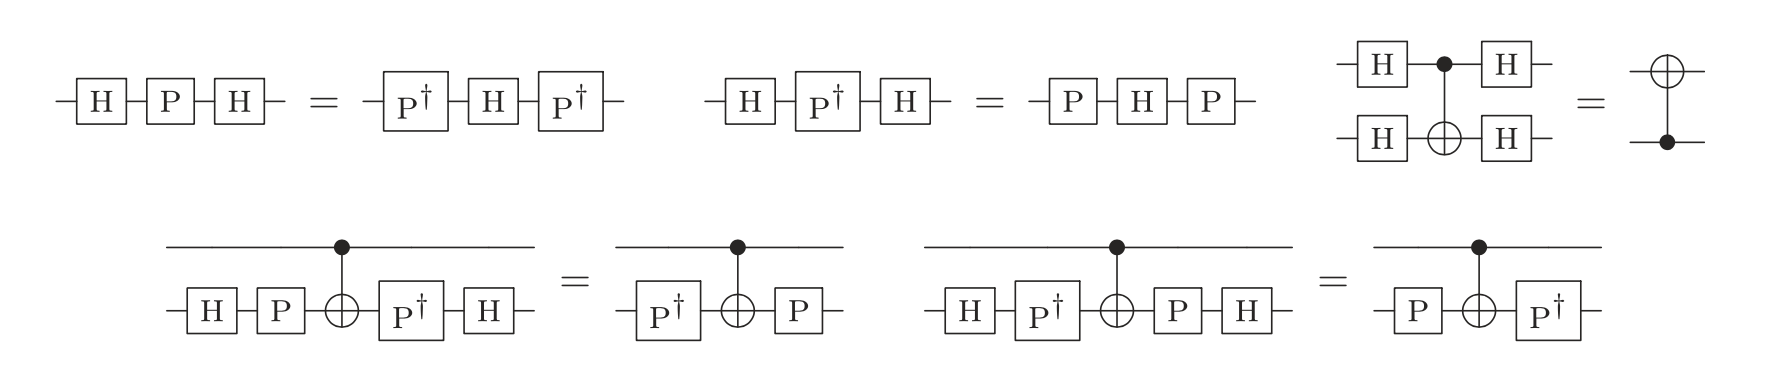
\includegraphics[width=0.9\linewidth]{images/hardmard_reduction.png}
            \caption{Subcircuit patterns in Hardmard Reduction}
        \end{figure}
    \end{center}

    \subsubsection{Gate Cancellation}
    When a pair of conjugate transpose gates are adjacent, they can both be cancelled.

    In this section, we implement gate cancellation for $RZ$ gate, we traverse all $RZ$ gates and try to move it by swap with adjacent commutative subcircuit if posible (we only consider serveral  built-in commutation rules (\ref{commutation}) since it is hard to determine whether two gates are commutative) until encountering its conjugate transpose or reaching endpoints of the circuit.

    \begin{center}
        \begin{figure}
            \label{commutation}
            \centering
            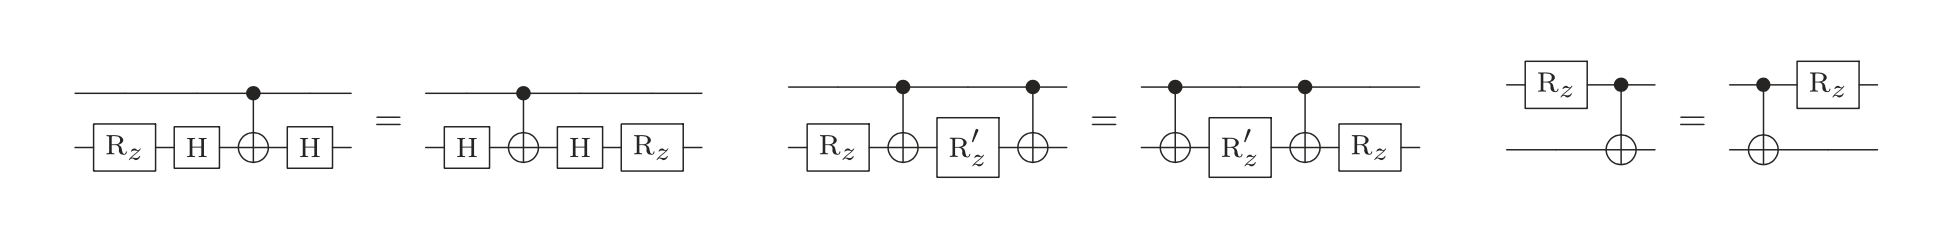
\includegraphics[width=0.9\linewidth]{images/gate_cancellation.png}
            \caption{Commutation rules for RZ gate}
        \end{figure}
    \end{center}

